\section{Evaluation}
\label{sec:evaluation}

\subsection{Experimental Setup}
\label{sec:evaluation.setup}

We implemented our monitoring architecture for adjustable overheads by
modifying the ARM version of the gem5 simulator \cite{gem5} to support parallel
run-time monitoring. We model the main and monitoring cores as running at 2.5
GHz with 4-way set-associative private L1 I/D caches and a shared 8-way 2 MB L2
cache. This setup is similar to the Snapdragon 801 processor commonly found in
mobile systems. The dataflow engine uses a 1 kB cache for flags.

In order to explore the generality of the architecture for
different monitors, we implemented three different monitors: uninitialized
memory check (UMC), array bounds check (BC), and dynamic information flow
tracking (DIFT).  Uninitialized memory check seeks to detect loading from
memory locations that are not initialized first.  Array bounds check, as
mentioned in Section~\ref{sec:monitoring} is a monitoring scheme that aims to
detect buffer overflows where memory accesses go beyond the boundaries of an
array. We modify the implementation of {\tt malloc} to set base and bound
metadata information. Dynamic information flow tracking is a security
monitoring scheme,
which detects when information from untrusted sources is used to affect the
program control flow. For our DIFT implementation, we set mark data read from
files as untrusted. This data is marked with a 32-bit metadata identifier so
that if an error is detected, it is possible to have information about where
the information originated from. 

We tested our system using all C benchmarks from SPECint
CPU2006 \cite{spec2006}. We focus on the C benchmarks because of our
modification of {\tt malloc} to support array bounds check. Although we do not
show results for the C++ benchmarks, we note that the results for UMC and DIFT
for these benchmarks are similar to the other results shown. For each
benchmark, we simulated for 200 million
instructions. An initial slack of 2 million cycles, which is less than 1\% of
the total execution time, is given for a 10\% target overhead. This initial
slack is scaled proportionally for other overhead targets.

\subsection{Baseline Monitoring Overheads}
% Full monitoring overheads
\begin{figure}
  \begin{center}
    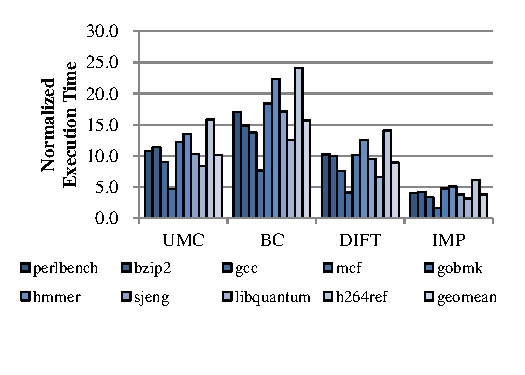
\includegraphics[width=\columnwidth]{figs/data_full_mon.pdf}
    \vspace{-0.2in}
    \caption{Full monitoring overheads for UMC, BC, and DIFT.}
    \label{fig:evaluation.full_mon}
    \vspace{-0.1in}
  \end{center}
\end{figure} Figure~\ref{fig:evaluation.full_mon} shows the execution times of
performing full monitoring normalized to the execution times of the benchmarks
without monitoring. In these results, no filtering or partial monitoring is
done. UMC shows normalized execution times from 5x to 11x with an average
of 8x. BC shows normalized execution times of 15-28x with an average of
22x while DIFT shows normalized execution times of 11x-17x with an average of
14x. One of the reasons for these high overheads is that our implementations of
these monitors dynamically allocate memory for new metadata. This can be an
expensive, multi-cycle operation. Statically allocating memory for metadata
will reduce the execution time but requires a large upfront memory footprint.

\subsection{Filtering of Monitoring Events}

% Full monitoring overheads
\begin{figure}
  \begin{center}
    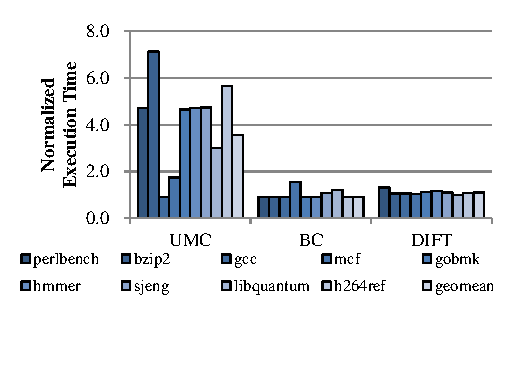
\includegraphics[width=\columnwidth]{figs/data_filtering.pdf}
    \vspace{-0.2in}
    \caption{Monitoring overheads with filtering for UMC, BC, and DIFT.}
    \label{fig:evaluation.filtering}
    \vspace{-0.1in}
  \end{center}
\end{figure}

Figure~\ref{fig:evaluation.filtering} shows the
normalized execution times with filtering enabled. We see significant
reductions in overhead for all three monitoring schemes. UMC sees normalized
execution times of 4x on average with filtering. For BC, normalized execution
times drop from 21x down to 3x. This is not surprising since in the baseline
implementation all loads and stores needed to be monitored. However, with
filtering, only loads and stores corresponding to arrays need to be forwarded.
Finally, DIFT sees the largest reduction in overheads with only 13\% overheads
on average. This is due to the fact that for our implementation of DIFT on SPEC
benchmarks, we mark data read from files as tainted. For most of these
benchmarks, this propagates to relatively few instructions. Instead, if we
targeted network or streaming applications we would expect to see a less
filtering

\subsection{Coverage with Adjustable Overheads}

% BC sweep
\begin{figure*}
  \begin{center}
    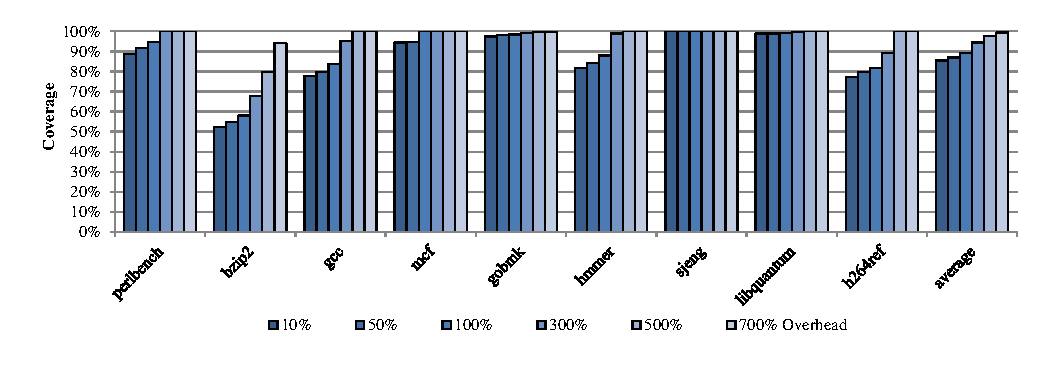
\includegraphics[width=\linewidth]{figs/data_bc_sweep.pdf}
    \vspace{-0.4in}
    \caption{Coverage versus varying overhead budget for array bounds check.}
    \label{fig:evaluation.bc_sweep}
    \vspace{-0.2in}
  \end{center}
\end{figure*}

% UMC sweep
\begin{figure*}
  \begin{center}
    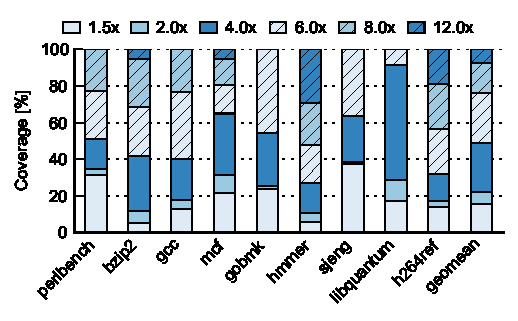
\includegraphics[width=\linewidth]{figs/data_umc_sweep.pdf}
    \vspace{-0.4in}
    \caption{Coverage versus varying overhead budget for uninitialized memory check.}
    \label{fig:evaluation.umc_sweep}
    \vspace{-0.1in}
  \end{center}
\end{figure*}

Although the overheads of DIFT are quite low after filtering, BC and UMC still
show significant overheads. In this section, we evaluate the effectiveness of
using partial monitoring to trade-off coverage for further reduced overheads.
Figure~\ref{fig:evaluation.bc_sweep} shows the monitoring coverage achieved by
array bounds check as we vary the overhead budget. We measure monitoring
coverage monitoring check operations that are still performed as a percentage
of the total number of monitoring check operations. This number does not
include the number metadata update operations that are done and serves as a
better metric for the actual coverage of the security or reliability technique.
The overhead is measured as a percentage of the program without monitoring. An
unrestricted dropping policy is used here.

We see that by varying the overhead budget, the coverage achieved also varies.
Furthermore, with only a 50\% overhead budget, array bounds check still
achieves 87\% monitoring coverage on average. This overhead budget corresponds
to 26\% of the average overheads seen by BC after filtering. The high coverage
achieved with such low overheads is due to two main effects.  The first is that
monitoring can be done in parallel, providing monitoring coverage without
introducing overheads. The second effect is that, although we aggressively
filter out monitoring events, there may still exist a large number of
monitoring events that do not lead to security or reliability checks. As a
result, dropping these events can reduce overheads without a large impact on
monitoring coverage.

Figure~\ref{fig:evaluation.umc_sweep} shows the analogous graph for UMC. Again
we see that varying overhead budgets enables partial monitoring. We see that
with a 50\% overhead budget, UMC achieves 50\% monitoring coverage on average.
This overhead budget corresponds to only 15\% of the overheads seen by UMC
after filtering.

\subsection{Comparing Dropping Policies}

In this section we evaluate the trade-offs of the three dropping policies
presented in Section~\ref{sec:policies.events}: unrestricted dropping, source
dropping, and sub-flow dropping.

% BC exec time
\begin{figure}
  \begin{center}
    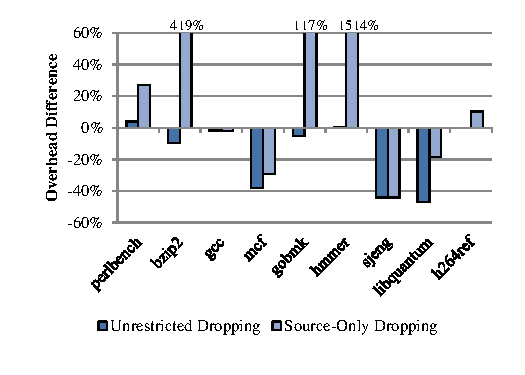
\includegraphics[width=\columnwidth]{figs/data_bc_exec_time.pdf}
    \vspace{-0.2in}
    \caption{Error in meeting overhead budget for array bounds check.}
    \label{fig:evaluation.bc_exec_time}
    \vspace{-0.2in}
  \end{center}
\end{figure}

% UMC exec time
\begin{figure}
  \begin{center}
    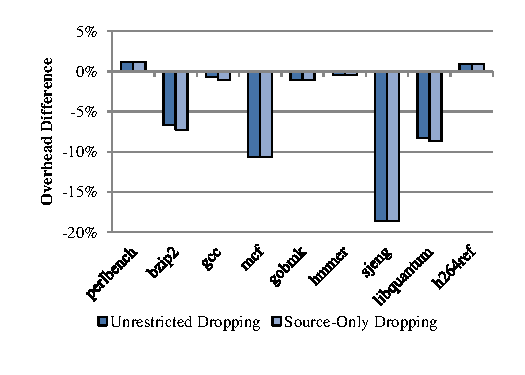
\includegraphics[width=\columnwidth]{figs/data_umc_exec_time.pdf}
    \vspace{-0.2in}
    \caption{Error in meeting overhead budget for uninitialized memory check.}
    \label{fig:evaluation.umc_exec_time}
    \vspace{-0.2in}
  \end{center}
\end{figure}

First, we evaluate how well the different policies are able to meet a specified
overhead budget. Figures~\ref{fig:evaluation.bc_exec_time} and
\ref{fig:evaluation.umc_exec_time} show the difference between the run-time
overheads seen and the overhead specified. These errors are averaged over all
benchmarks. A positive value means that the
overhead target was overshot while a negative value indicates that the
overheads were below the specified budget.

% BC coverage across policies
\begin{figure}
  \begin{center}
    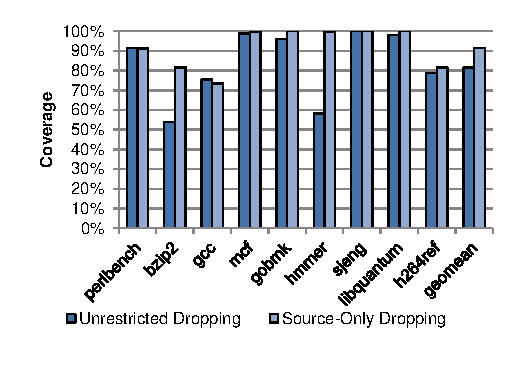
\includegraphics[width=\columnwidth]{figs/data_bc_coverage.pdf}
    \vspace{-0.2in}
    \caption{Coverage for array bounds check for different dropping policies.}
    \label{fig:evaluation.bc_coverage}
    \vspace{-0.2in}
  \end{center}
\end{figure}

% UMC coverage across policies
\begin{figure}
  \begin{center}
    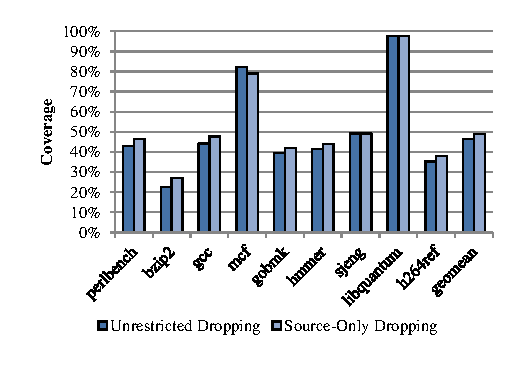
\includegraphics[width=\columnwidth]{figs/data_umc_coverage.pdf}
    \vspace{-0.2in}
    \caption{Coverage for uninitialized memory check for different dropping policies.}
    \label{fig:evaluation.umc_coverage}
    \vspace{-0.1in}
  \end{center}
\end{figure}

Next, we evaluate the coverage achieved by the different policies.
Figure~\ref{fig:evaluation.bc_coverage} shows the average coverage across
benchmarks for each of the three policies with varying overhead budgets.
Figure~\ref{fig:evaluation.umc_coverage} shows this data for uninitialized
memory check.

\subsection{Area and Power Overheads}

% Area and Power Overheads
\begin{table}[tb]
  \begin{center}
    \vspace{-0.0in}
    \begin{footnotesize}
    
% Full monitoring at zero slack

\begin{tabular}{|c|c|c|}
\hline

{\bf Monitor} & {\bf Peak Power [mW]} & {\bf Runtime Power [mW]} \\ \hline\hline

UMC  & 4.7 (4.9\%) &  3.1 (8.2\%) \\ \hline
BC   & 6.9 (7.1\%) &  4.1 (10.7\%) \\ \hline
DIFT & 7.2 (7.4\%) &  4.3 (11.1\%) \\ \hline

\end{tabular}

    \end{footnotesize}
    \caption{Average power overhead for dropping hardware at a 10\% overhead
    budget. Percentages in parentheses are normalized to the main core
    power.}
    \vspace{-0.2in}
    \label{tab:evaluation.area_power}
  \end{center}
\end{table}

Adding the dropping hardware in order to enable adjustable overheads adds
overheads in terms of area and power. We use McPat \cite{mcpat-micro09} to get
a first-order estimate of these area and power overheads in a 40 nm technology
node. McPat estimates the main core area as 1.96 mm$^2$ and the peak power usage as
121 mW averaged across all benchmarks. The average runtime power usage was 38.2 
mW. These area and power numbers consist of the core and
L1 cache, but do not include L2 cache, memory controller, and other
peripherals. The power numbers include dynamic as well as static (leakage)
power. For the dropping hardware, the ALUs, MIRF, MIC, and
configuration tables are modeled using the corresponding objects in McPat. We
note that this is only a rough area and power result since components such as the
wires connecting these modules have not been modeled. However, this gives a
sense of the order-of-magnitude overheads involved with implementing our
approach.

For a 1 kB MIC, an additional 0.183 mm$^2$ of silicon area is needed, an
increase of 9\% of the main core area. Table~\ref{tab:evaluation.area_power}
shows the peak and runtime power overheads. The peak power is 13-19 mW, which is
11-16\% of the main core's peak power usage. The average runtime power is 8-11
mW, corresponding to 21-29\% of the main core's runtime power.

